\chapter{Experiments}
%TODO: explain statistical method: precission, recall, f1, density

For the final quantitative evaluation formulate a series of experiments and then perform a statistical hypothesis testing. 
We use our resulting segmentations as a prediction and compare it against a predefined ground truth. 


Our random variable 

For this purpose we introduce a binary random variable, indicating whether a particular sampling point is assigned to the correct ground truth segment.

To illustrate the concept of hypothesis testing let discuss the follo


X = suffers from deadly infection
TP: a person suffers from a particular infection and was detected. person can be cured and won't infect other person.
FN: a person suffers from a infection and was not detected. thus might infect other people. bad scenario
FP: a person is healthy but was incorrectly diagnosed being ill. person will be treated even though it is healthy. bad scenario
TN: a person is healthy and was actually diagnosed like that. everything is okay.


Sensitivity and specificity are statistical measures of the performance of a binary classification test, also known in statistics as classification function:

  Sensitivity (also called the true positive rate, or the recall in some fields) measures the proportion of positives that are correctly identified as such (e.g., the percentage of sick people who are correctly identified as having the condition).
    Specificity (also called the true negative rate) measures the proportion of negatives that are correctly identified as such (e.g., the percentage of healthy people who are correctly identified as not having the condition).


    
For the final quantitative evaluation of our experiments we make use of the F1 measure. This measure is often used in determining the performance of  classification tasks in machine learning. To compute its score, this measure takes into account both, the precission and the recall of the test. 
 The exact definition of the F1 measure is given in equation $\ref{eq:f1_score}$.
\begin{equation}
F_1 = 2 \left( \frac{\text{preccision} \times \text{recall}}{\text{preccision} +\text{recall}} \right)
\label{eq:f1_score}
\end{equation}  
The F1 score can be interpreted as a normalized weighted average of the precision and recall test performances. The best possible F1 score is equals 1 and its worst value is 0.
    
\begin{table}[H]
\centering
\begin{tabular}{c|c|c|}
\cline{2-3}
 & \begin{tabular}[c]{@{}l@{}}Prediction\\ Positive\end{tabular} & \begin{tabular}[c]{@{}l@{}}Prediction\\ Negative\end{tabular} \\ \hline
\multicolumn{1}{|l|}{\begin{tabular}[c]{@{}l@{}}Condition\\ Positive\end{tabular}} & \cellcolor[HTML]{34FF34}{\color[HTML]{000000} $\bf{TP}$ } & \cellcolor[HTML]{CB0000} $\bf{FN}$ \\ \hline
\multicolumn{1}{|l|}{\begin{tabular}[c]{@{}l@{}}Condiation\\ Negative\end{tabular}} & \cellcolor[HTML]{CB0000}{\color[HTML]{000000} $\bf{FP}$ } & \cellcolor[HTML]{34FF34} $\bf{TN}$ \\ \hline
\end{tabular}
\caption[Prediction and Sensivity]{My caption}
\label{tab:prediction_sensitivity}
\end{table}

\begin{figure}[H]
\begin{center}
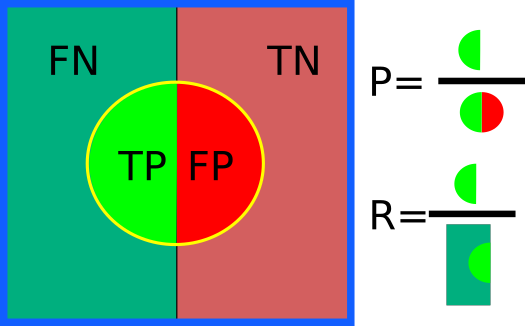
\includegraphics[width=0.6\linewidth] {evaluation/prec_recall}
\end{center}
\caption[Concept Recall and Precision]{This figure illustrates graphically the concept of Recall (\textbf{R}) and Precision (\textbf{P}). When estimating the sampling of a binary random variable, there are basically four possible outcomes: The we predicted it being true and it is true (\textbf{TP}), we predicted it true but it is false (\textbf{FP}), we predicted it false and it was actually negative (\textbf{FN}) or we predicted it to be true but it was actually false (\textbf{TN}). }
\label{fig:eval_concept_recall_precc}
\end{figure}



\section{Datasets}
\label{sec:datasets}




\begin{table}[H]
\centering
\begin{tabular}{|l|l|l|l|l|}
\hline
\textbf{Dataset} & \textbf{\#Frames} & \textbf{Resolution} & \textbf{Has Depths} & \textbf{Cameras Aligned} \\ \hline
cars & 19 & 480 x 640 & false & false \\ \hline
wh & 104 & 480 x 640 & true & false \\ \hline
bonn\_chairs & 58 & 480 x 640 & true & true \\ \hline
bonn\_watercan & 58 & 480 x 640 & true & true \\ \hline
bonn\_cerealbox & 101 & 480 x 640 & true & true \\ \hline
alley2 & 50 & 512 x 218 & true & true \\ \hline
two\_chairs & 61 & 512 x 424 & true & true \\ \hline
chair & 101 & 512 x 424 & true & true \\ \hline
\end{tabular}
\caption[Datasets]{Properties of our used datasets.}
\label{tab:datasets}
\end{table}


make table similar to github redme about dataset
display first,center and last frame per dataset

\section{Parameterspace Exploration}
\subsection{Influence of $\lambda$}

\begin{figure}[H]
\centering
\begin{tikzpicture}[trim axis left]
\begin{axis}[
  axis x line=center,
  axis y line=center,
  grid=both,
  xtick={-1,...,10},
  ytick={-1,...,10},
  xlabel={$x$},
  ylabel={$e^{-\lambda d}$},
  xlabel style={below right},
  ylabel style={above left},
  no markers,
  xmin=-0.5,
  xmax=1.5,
  ymin=-1.5,
  ymax=1.5]
\addplot +[thick, domain=0:10] {exp(-x)};
\end{axis}
\end{tikzpicture}
\caption[Affinity Function]{A plot of the affinity transformation function. We observe that the smaller the $\lambda$ paramter gets, the larger the affinities become and wise versa.}
\label{fig:exp_effect_lambda}
\end{figure}


\begin{figure}[H]
\begin{center}

\subfigure[$\lambda = 1$]{
   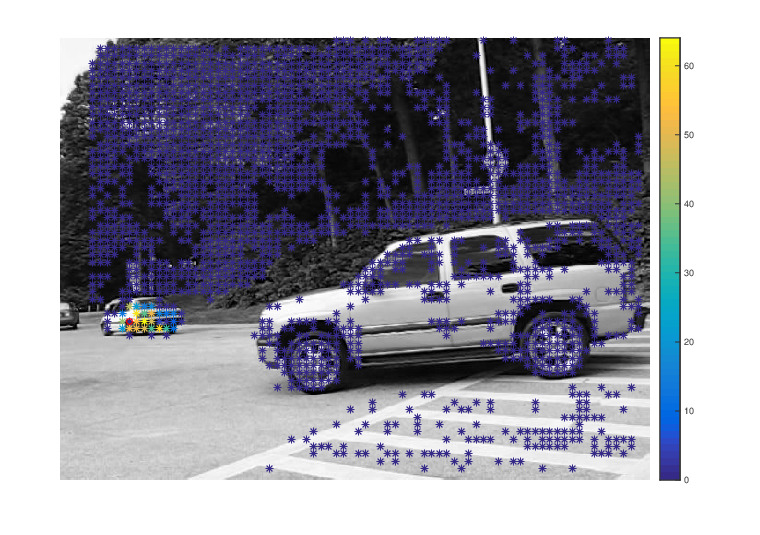
\includegraphics[width=0.48\linewidth] {evaluation/effect_of_lambda/cars_lambda_1}
   \label{fig:cars_eff_lam_a}
}
\subfigure[$\lambda = 0.1$]{
   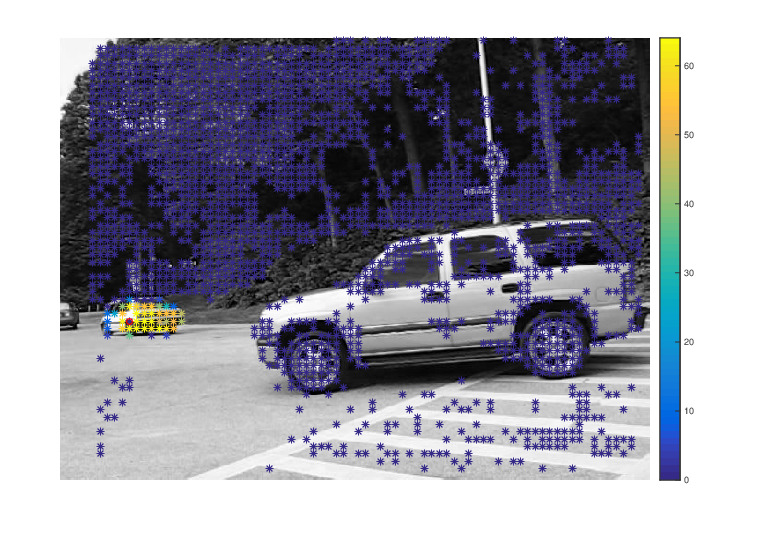
\includegraphics[width=0.48\linewidth] {evaluation/effect_of_lambda/cars_lambda_0_1}
   \label{fig:cars_eff_lam_b}
}
~
\subfigure[$\lambda = 0.01$]{
   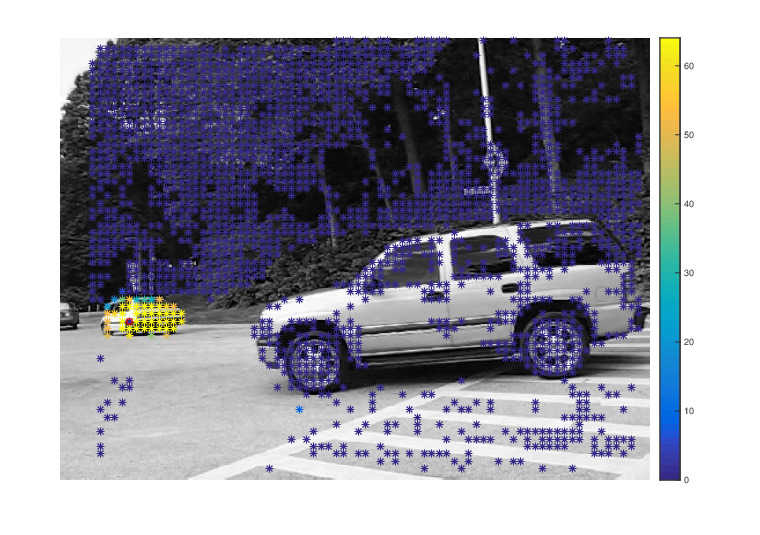
\includegraphics[width=0.48\linewidth] {evaluation/effect_of_lambda/cars_lambda_0_01}
   \label{fig:cars_eff_lam_b}
}
\subfigure[$\lambda = 0.001$]{
   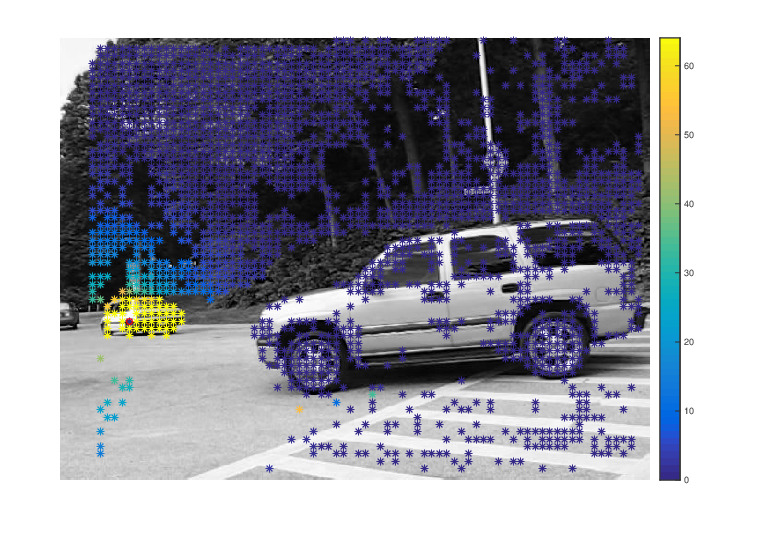
\includegraphics[width=0.48\linewidth] {evaluation/effect_of_lambda/cars_lambda_0_001}
   \label{fig:cars_eff_lam_b}   
}
\end{center}
\caption[Influence of Lambda Parameter]{Illustration of the influence of the $\lambda$ parameter used for computing trajectory affinities. A plot of the affinity transformation function is shown in figure $\ref{fig:exp_effect_lambda}$. }
\label{fig:cars_effect_of_lambda}
\end{figure}

\section{Qualitative Evaluation}
mention available pipeline levels and their main parameters again
tracking candidates

\section{Quantitative Evaluation}


%TODO: statistics: performance of selected set of methods applied on all datasets: HS_PD_SC, LDOF_PD_SC (classic), LDOF_PED_MC, LDOF_SD, LDOF_SED, SRSF_PED, SRSF_SED
%TODO: statistics: influence of lambda using LDOF_PD
%TODO: statistics: LDOF_PED_SC vs LDOF_PD_SC
%TODO: statistics: LDOF_PED_SC vs LDOF_PED_SC
%TODO: statistics: LDOF_PD_MC vs LDOF_SD
%TODO: statistics: LDOF_PED_MC vs LDOF_SED
%TODO: statistics: best case - tweak paras for a dataset.

method comparison, given a fixed number of clusters

\subsection{Evaluation of Datasets}
mention that we use merged clusters for performing the evaluations.


\subsubsection{Bonn Chairs}
% TODO: update results according to the new mask:
% particularly, mention the following observations:
% ldof flow perform poor, since they are not able to successfully segment the lower chair part. this might be due to many reasons:
% on one hand, trajectories have to be relatively robust similar to each other to prevent oversegmentation potentially resulting from rotational movements. On the other hand, the movement of the lower chair segment strongly correlates with the upper (seat, lean) segment. Moreover, trajectories within this lower chair region are not very accurate due to shadows and lightning conditions.
% TODO: compare impact of results when using a complete chair mask
% TODO: compare results when using SRSF flows

The \textit{Bonn Chairs} dataset is a video sequence consisting of 58 frames. It shows a room containing two chairs and a man. The man is moving the and rotating the right chair. Also, the camera is moving. See figure $\ref{fig:eval_bonn_chairs_frames}$ to get a better understanding of the whole scene.
\begin{figure}[H]
\begin{center}
\subfigure[Frame 1]{
   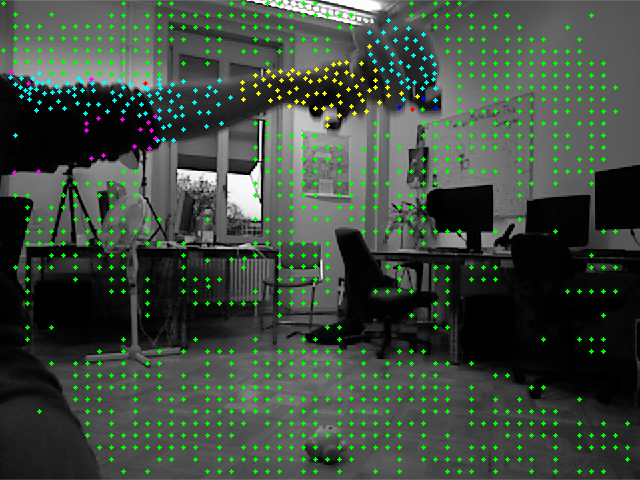
\includegraphics[width=0.31\linewidth] {evaluation/bonn_chairs_frames/1}
   \label{fig:eval_bonn_chairs_frames_a}
}
\subfigure[Frame 12]{
   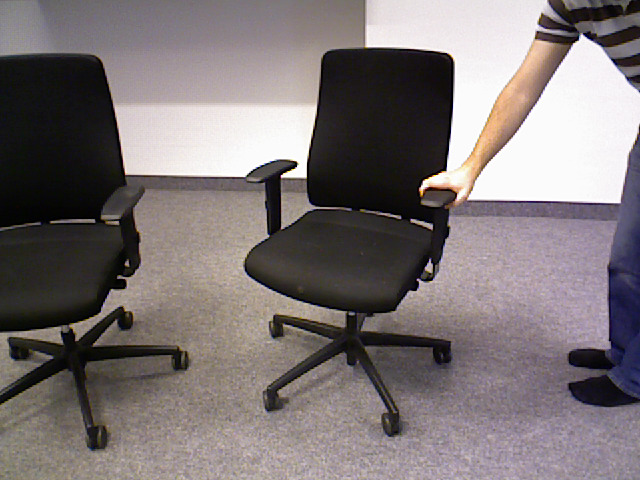
\includegraphics[width=0.31\linewidth] {evaluation/bonn_chairs_frames/12}
   \label{fig:eval_bonn_chairs_frames_b}
}
\subfigure[Frame 24]{
   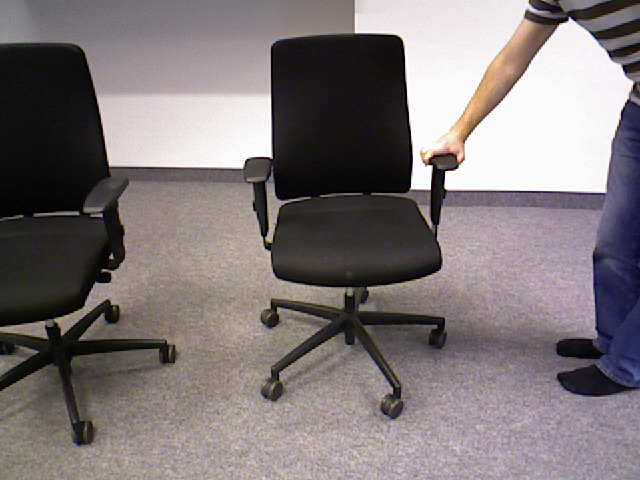
\includegraphics[width=0.31\linewidth] {evaluation/bonn_chairs_frames/24}
   \label{fig:eval_bonn_chairs_frames_c}
}
~
\subfigure[Frame 35]{
   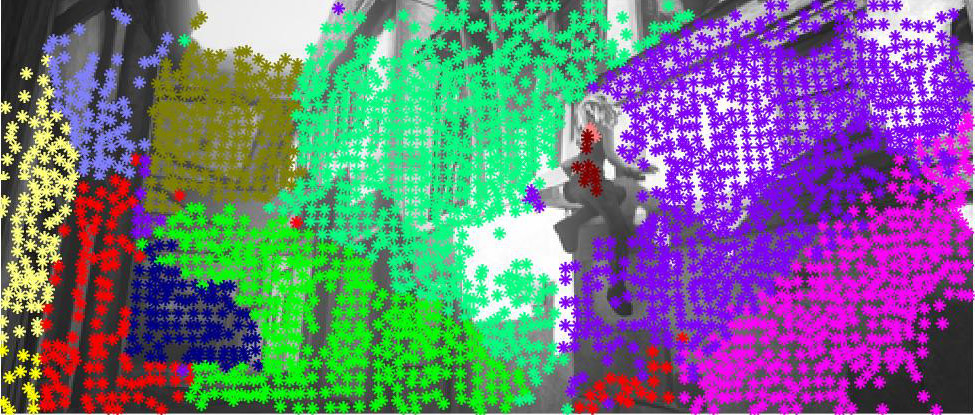
\includegraphics[width=0.31\linewidth] {evaluation/bonn_chairs_frames/35}
   \label{fig:eval_bonn_chairs_frames_a}
}
\subfigure[Frame 47]{
   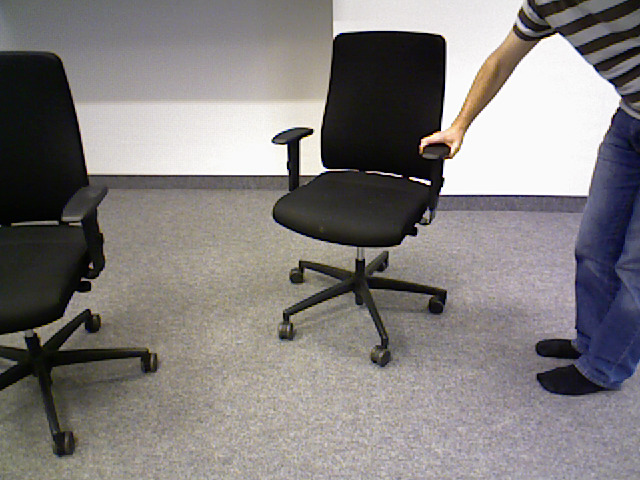
\includegraphics[width=0.31\linewidth] {evaluation/bonn_chairs_frames/47}
   \label{fig:eval_bonn_chairs_frames_b}
}
\subfigure[Frame 58]{
   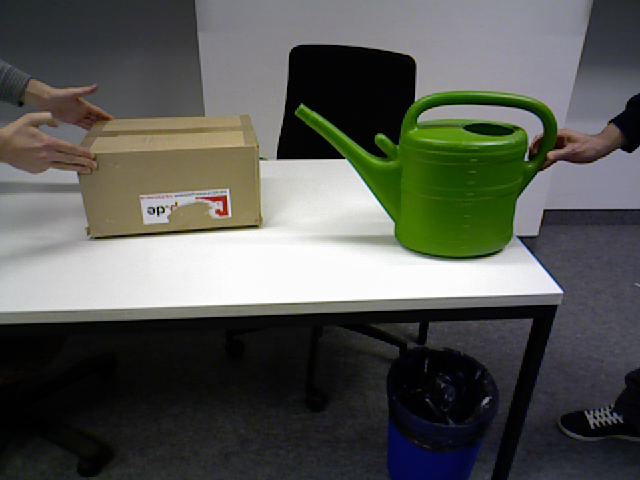
\includegraphics[width=0.31\linewidth] {evaluation/bonn_chairs_frames/58}
   \label{fig:eval_bonn_chairs_frames_c}
}
\end{center}
\caption[Bonn Chairs Dataset]{Listing of 6 ascending frames of the our Bonn Chairs dataset. In this dataset we have a scene in which there are 2 chairs and a man in a room. The man is moving and rotating the right chair. The same time, also the camera is slightly moving around.}
\label{fig:eval_bonn_chairs_frames}
\end{figure}
This dataset contains depth images as well as camera calibration data. The depth-and color camera are already aligned. \\ \\
For the following experiment we only use LDOF flows. Moreover, we fix the number of clusters we want to solve for and set it equal to six segments. In our pipeline we run all valid cross combinations between our affinity computation methods, such as PD, PED, SD and SED and the segmentation methods SC, MC and KL. The resulting segmentations are shown in figure $\ref{fig:eval_bonn_chairs_raw_segmentations}$. 
\begin{figure}[H]
\begin{center}
\subfigure[LDOF PD SC]{
   \includegraphics[width=0.48\linewidth] {evaluation/bonn_chairs_segmentations_raw_f_20/ldof_pd_sc}
   \label{fig:eval_bonn_chairs_raw_segmentations_a}
}
\subfigure[LDOF PD MC]{
   \includegraphics[width=0.48\linewidth] {evaluation/bonn_chairs_segmentations_raw_f_20/ldof_pd_mc}
   \label{fig:eval_bonn_chairs_raw_segmentations_b}
}
~
\subfigure[LDOF PED SC]{
   \includegraphics[width=0.48\linewidth] {evaluation/bonn_chairs_segmentations_raw_f_20/ldof_ped_sc}
   \label{fig:eval_bonn_chairs_raw_segmentations_c}
}
\subfigure[LDOF PED MC]{
   \includegraphics[width=0.48\linewidth] {evaluation/bonn_chairs_segmentations_raw_f_20/ldof_ped_mc}
   \label{fig:eval_bonn_chairs_raw_segmentations_d}
}
~
\subfigure[LDOF SD KL]{
   \includegraphics[width=0.48\linewidth] {evaluation/bonn_chairs_segmentations_raw_f_20/ldof_sd_kl}
   \label{fig:eval_bonn_chairs_raw_segmentations_e}
}
\subfigure[LDOF SED** KL]{
   \includegraphics[width=0.48\linewidth] {evaluation/bonn_chairs_segmentations_raw_f_20/ldof_sed_kl}
   \label{fig:eval_bonn_chairs_raw_segmentations_f}
}
\end{center}
\caption[Bonn Chairs Segmentations]{Segmentations produced by our pipeline when running the Bonn Chairs dataset, using six cluster.}
\label{fig:eval_bonn_chairs_raw_segmentations}
\end{figure}
Ideally, a segmentation should have a separate mask for the man's arm, the lower parts (the seat and the star base) of the office chair and its backrest, as well as one for the background.

At a first glance, are methods were performing rather well, being capable of detecting all these expected masks. However, there is still a difference in the their result's quality. Especially around the region of the men's arm, we observe a difference of quality when comparing methods that make use of depth information with those not making use of any depth. Non-depth using methods tend to assign points to the arm's cluster which should belong to the background. This could however be due to the fact that such points are spatially close to the arm and thus exhibit a large affinity value to the trajectories within the arm region. \\ \\
Interestingly, the SD KL method was oversegmenting the chair's seat into two clusters. One possible explanation for this could be, that we were using a too large probability value when using six clusters. \\ \\
Some methods seem to have trouble in correctly segmenting the chair's arm lean, especially all MC clustering methods seem to have issues in correctly assigning this region. \\ \\
Last, please notice that we used many more cluster for the SED KL method, since it performed very poor when using six clusters. The actual result when using 6 only six clusters is shown in figure $\ref{fig:bonn_chairs_sed_varyingclusters}$. The reason why we legitimate ourself to use this 10 cluster result is stated below.

STATE SOME QUALITATIVE OBSERVATIONS HERE. \\ \\

For measuring the quantitative performance of the resulting segmentations we compare their merged cluster versions, which are shown in figure $\ref{fig:eval_bonn_chairs}$, with the ground truth mask as depcited in figure $\ref{fig:eval_bonn_chairs_gt_20}$.
\begin{figure}[H]
\begin{center}
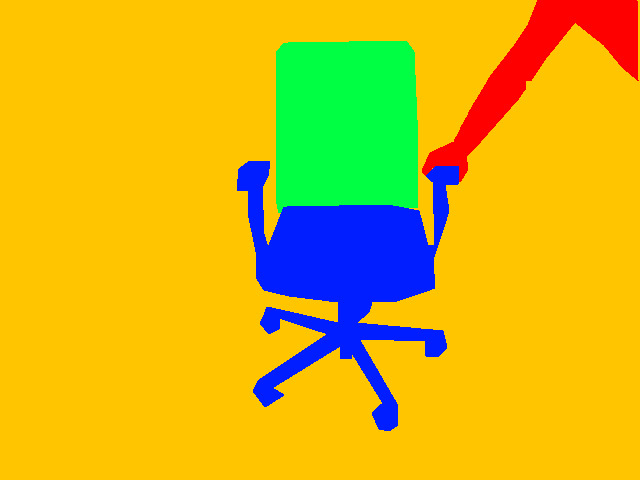
\includegraphics[width=0.48\linewidth] {evaluation/bonn_chairs/gt_20}
\end{center}
\caption[Bonn Chairs GT Frame 20]{Ground truth frame No. 20 of the Bonn Chairs dataset.}
\label{fig:eval_bonn_chairs_gt_20}
\end{figure}
Quantitative evaluations are listed in table $\ref{tab:eval_bonn_chairs}$. 
\begin{table}[H]
\centering
\begin{tabular}{|l|l|r|l|l|l|}
\hline
\multicolumn{6}{|c|}{Comparison bonn chairs dataset using 6 clusters}                        \\ \hline
              & \textbf{Density} & \textbf{Precision} & \textbf{Recall} & \textbf{F1 Score} & \textbf{Fragmentation} \\ \hline
LDOF PD SC & 0.43685 & 86.2087 \%   & 76.607 \%     & 81.1247 \%  & x \% \\ \hline
LDOF PD MC & 0.43685 & 86.4193 \%   & 76.1967 \%     & 80.9867 \%  & x \%   \\ \hline
LDOF PED SC & 0.37174 & 95.0959 \%   & 78.1937 \%     & 85.8205 \%  & x \%   \\ \hline
LDOF PED MC & 0.37174 & 83.3878 \%   & 91.4203 \%     & 87.2195 \%  & x \%   \\ \hline              
LDOF SD KL & 0.43848 & 74.7623 \%   & \textbf{96.4264} \%     & 84.2235 \%  & x \%   \\ \hline
LDOF SED KL & 0.37402 & 38.5505 \%   & 66.0331 \%     & 48.6809 \%  & x \%   \\ \hline
LDOF $\text{SED}^{*}$ KL & 0.37402 & 73.8535 \%   & 94.4836 \%     & 82.9045 \%   & x \%  \\ \hline
LDOF $\text{SED}^{**}$ KL & 0.37402 & $\textbf{96.1708}$ \%   & 89.9521 \%     & $\textbf{92.9576}$ \%    & x \%  \\ \hline
\end{tabular}
\caption[Cars Dataset]{Quantitative evaluation of the bonn chairs dataset using the LDOF flow method. Note that there are two additional evaluations for the SED method available, indicated by * and **. The * variant was run using 9 clusters and the ** was run using 10 clusters. The reason for doing so was that the parameter space was simply too large to find the optimal parameter to obtain no oversegmentation. See figure $\ref{fig:bonn_chairs_sed_varyingclusters}$.}
\label{tab:eval_bonn_chairs}
\end{table}
We clearly observe, that as soon as we make use of depth informations, the F1 measure increases drastically. Additionally, the summed distances (SD, SED) outperform product distances (PD,PED). The merged segmentations used for the evaluation are shown in figure $\ref{fig:eval_bonn_chairs}$. \\ \\
\begin{figure}[H]
\begin{center}
\subfigure[LDOF PD SC]{
   \includegraphics[width=0.48\linewidth] {evaluation/bonn_chairs/ldof_pd_sc}
   \label{fig:bonn_chairs_b}
}
\subfigure[LDOF PD MC]{
   \includegraphics[width=0.48\linewidth] {evaluation/bonn_chairs/ldof_pd_mc}
   \label{fig:bonn_chairs_c}
}
~
\subfigure[LDOF PED SC]{
   \includegraphics[width=0.48\linewidth] {evaluation/bonn_chairs/ldof_ped_sc}
   \label{fig:bonn_chairs_d}
}
\subfigure[LDOF PED MC]{
   \includegraphics[width=0.48\linewidth] {evaluation/bonn_chairs/ldof_ped_mc}
   \label{fig:bonn_chairs_e}
}
~
\subfigure[LDOF SD KL]{
   \includegraphics[width=0.48\linewidth] {evaluation/bonn_chairs/ldof_sd_kl}
   \label{fig:bonn_chairs_d}
}
\subfigure[LDOF SED** KL]{
   \includegraphics[width=0.48\linewidth] {evaluation/bonn_chairs/ldof_sed_kl}
   \label{fig:bonn_chairs_e}
}
\end{center}
\caption[Merged Segments Bonn Chairs]{Final, merged segmentation results of frame 20 when running our pipeline on the bonn dataset. The quantitive measures of these segmentations are listed in table $\ref{tab:eval_bonn_chairs}$.}
\label{fig:eval_bonn_chairs}
\end{figure}


% new bonn chairs fig
\begin{figure}[H]
\begin{center}
\subfigure[LDOF PD SC]{
   \includegraphics[width=0.48\linewidth] {evaluation/bonn_chairs_c_10/ldof_pd_sc}
   \label{fig:bonn_chairs_c_10_b}
}
\subfigure[LDOF PD MC]{
   \includegraphics[width=0.48\linewidth] {evaluation/bonn_chairs_c_10/ldof_pd_mc}
   \label{fig:bonn_chairs_c_10_c}
}
~
\subfigure[LDOF PED SC]{
   \includegraphics[width=0.48\linewidth] {evaluation/bonn_chairs_c_10/ldof_ped_sc}
   \label{fig:bonn_chairs_c_10_d}
}
\subfigure[LDOF PED MC]{
   \includegraphics[width=0.48\linewidth] {evaluation/bonn_chairs_c_10/ldof_ped_mc}
   \label{fig:bonn_chairs_c_10_e}
}
~
\subfigure[LDOF SD KL]{
   \includegraphics[width=0.48\linewidth] {evaluation/bonn_chairs_c_10/ldof_sd_kl}
   \label{fig:bonn_chairs_c_10_d}
}
\subfigure[LDOF SED KL]{
   \includegraphics[width=0.48\linewidth] {evaluation/bonn_chairs_c_10/ldof_sed_kl}
   \label{fig:bonn_chairs_c_10_e}
}
\end{center}
\caption[Merged Segments Bonn Chairs]{Final, merged segmentation results of frame 30 when running our pipeline on the bonn dataset. The quantitive measures of these segmentations are listed in table $\ref{tab:eval_bonn_chairs}$.}
\label{fig:eval_bonn_chairs_c_10}
\end{figure}
% end new bonn chairs fig

% new bc table
\begin{table}[H]
\centering
\begin{tabular}{|l|l|r|l|l|l|}
\hline
\multicolumn{6}{|c|}{Comparison bonn chairs dataset using 10 clusters}                        \\ \hline
              & \textbf{Density} & \textbf{Precision} & \textbf{Recall} & \textbf{F1 Score} & \textbf{Fragmentation} \\ \hline
LDOF PD SC & 0.43685 & 86.2087 \%   & 76.607 \%     & 81.1247 \%  & x \% \\ \hline
LDOF PD MC & 0.43685 & 86.4193 \%   & 76.1967 \%     & 80.9867 \%  & x \%   \\ \hline
LDOF PED SC & 0.37174 & 95.0959 \%   & 78.1937 \%     & 85.8205 \%  & x \%   \\ \hline
LDOF PED MC & 0.37174 & 83.3878 \%   & 91.4203 \%     & 87.2195 \%  & x \%   \\ \hline              
LDOF SD KL & 0.41146 / 0.42741 & 36.9619 / 21.1382 \%   & 27.5697 / 21.1382 \%     & 31.5823 / 21.1382 \%  & x \%   \\ \hline
LDOF SED KL & 0.37402 & $\textbf{96.1708}$ \%   & 89.9521 \%     & $\textbf{92.9576}$ \%    & x \%  \\ \hline
\end{tabular}
\caption[Bonn Chairs Merged 10 Clusters]{}
\label{tab:eval_bonn_chairs_c_10}
\end{table}
% end new bc table



Please notice that the performance of the $\textit{LDOF\_SED\_KL}$ is very poor for this cluster assignment. The reason for this is because this method was not well parameterized, resulting in a large oversegmentation. However, since this optimal parameter assignment exists, but was not found, we further investigated the performance by performing two additional experiments. The SED method was run, once using 9 clusters (indicated by SED* KL), and once again using 10 clusters (SED** KL). As we can see, the method LDOF SED** KL is superior compared to every other method run on this dataset. The actual segmentation results of the different SED methods are shown in figure $\ref{fig:bonn_chairs_sed_varyingclusters}$.






\begin{figure}[H]
\begin{center}
\subfigure[6 Clusters]{
   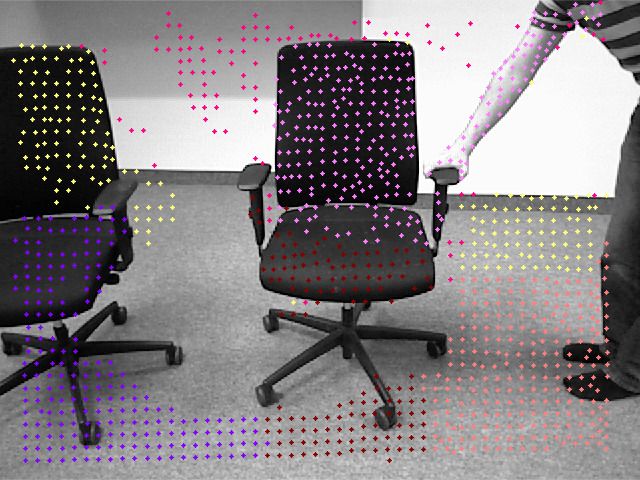
\includegraphics[width=0.31\linewidth] {evaluation/bonn_chair_ldof_sed/f_20_c_6}
   \label{fig:bonn_chairs_sed_varyingclusters_a}
}
\subfigure[9 Clusters]{
   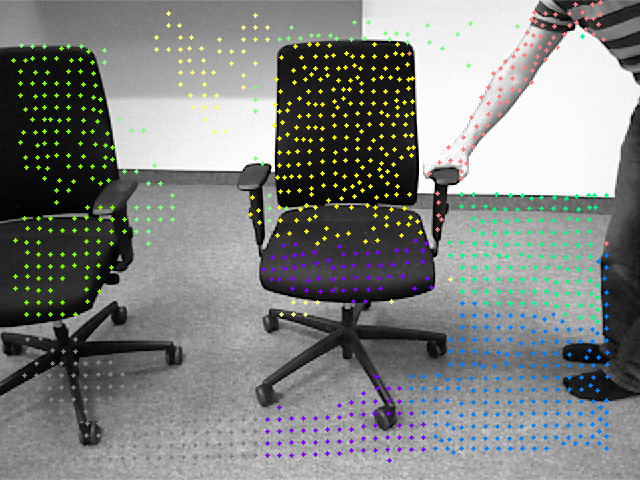
\includegraphics[width=0.31\linewidth] {evaluation/bonn_chair_ldof_sed/f_20_c_9}
   \label{fig:bonn_chairs_sed_varyingclusters_b}
}
\subfigure[10 Clusters]{
   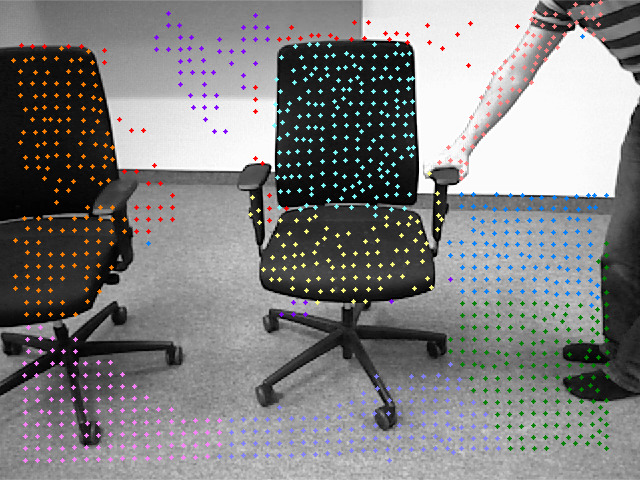
\includegraphics[width=0.31\linewidth] {evaluation/bonn_chair_ldof_sed/f_20_c_10}
   \label{fig:bonn_chairs_sed_varyingclusters_c}
}
\end{center}
\caption[Bonn Chairs SED Segmentations for Varying Cluster Count]{A visualization of the real segmentations when running \textit{SED KL} on the \textit{bonn chairs} dataset.}
\label{fig:bonn_chairs_sed_varyingclusters}
\end{figure}

%TODO mention some facts about the qualitative properties of the segmentations.

\subsubsection{Cars Dataset}


\begin{table}[H]
\centering
\begin{tabular}{|l|l|r|l|l|}
\hline
\multicolumn{5}{|c|}{Comparision cars dataset 3 clusters}                        \\ \hline
              & \textbf{Density} & \textbf{Precission} & \textbf{Recall} & \textbf{F1 Score} \\ \hline
LDOF PD SC & 0.66829 & 91.0544 \%   & 89.8432 \%     & 90.4447 \%  \\ \hline
LDOF PD MC & 0.66829 & 91.0502 \%   & 88.9107 \%     & 89.9677 \%  \\ \hline              
LDOF SD & 0.69987 & 79.2541 \%   & 92.709 \%     & 85.4551 \%  \\ \hline
\end{tabular}
\caption[Cars Dataset]{My caption}
\label{tab:cars_ldof_quality}
\end{table}

\begin{figure}[H]
\begin{center}

\subfigure[GT]{
   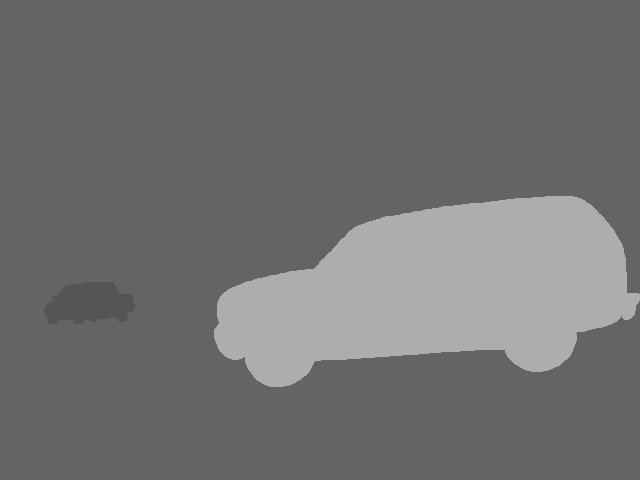
\includegraphics[width=0.48\linewidth] {evaluation/method_2d_ds/gt_1}
   \label{fig:cars_a}
}
\subfigure[LDOF PD SC]{
   \includegraphics[width=0.48\linewidth] {evaluation/method_2d_ds/ldof_pd_sc}
   \label{fig:cars_b}
}
~
\subfigure[LDOF PD MC]{
   \includegraphics[width=0.48\linewidth] {evaluation/method_2d_ds/ldof_pd_mc}
   \label{fig:cars_c}
}
\subfigure[LDOF SD]{
   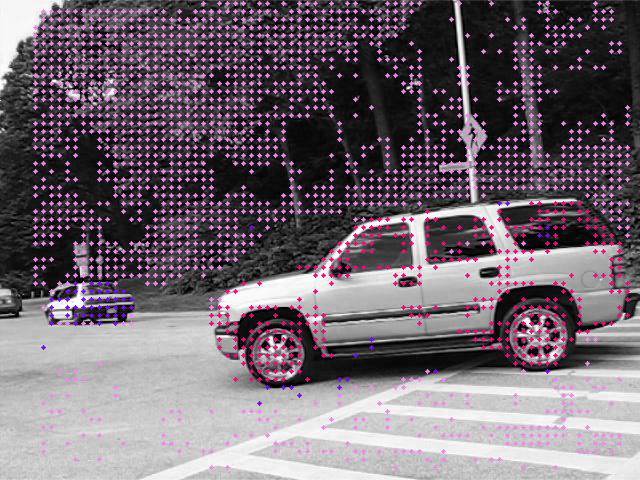
\includegraphics[width=0.48\linewidth] {evaluation/method_2d_ds/ldof_sd}
   \label{fig:cars_d}   
}
\end{center}
\caption[Method Comparison]{Visualization of segmentation resulting when running our pipeline on a dataset without depth information.}
\label{fig:cars_dataset}
\end{figure}



\subsubsection{Bonn Watercan Dataset}

dataset: bonn watercan
Fragmentation: 0.66667

\begin{figure}[H]
\begin{center}
\subfigure[GT Waterbox Frame 4]{
   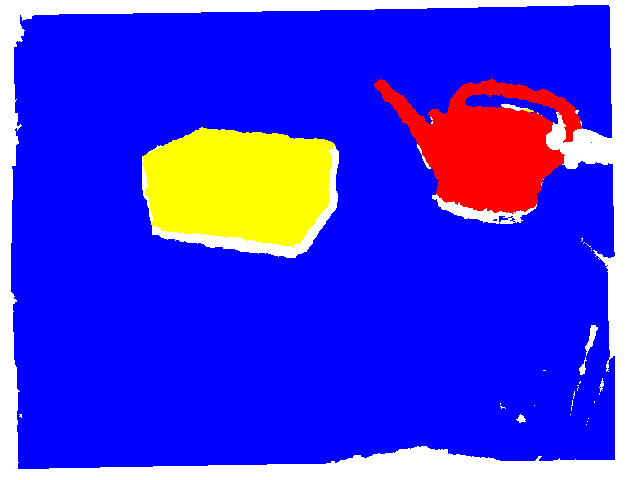
\includegraphics[width=0.7\linewidth] {evaluation/meth_cmp_bonn_wc/gt_4}
   \label{fig:bonn_gieskanne_gt}
}
~
\subfigure[LDOF PED SC]{
   \includegraphics[width=0.48\linewidth] {evaluation/meth_cmp_bonn_wc/ldof_ped_sc}
   \label{fig:bonn_wc_a}
}
\subfigure[LDOF PED SC]{
   \includegraphics[width=0.48\linewidth] {evaluation/meth_cmp_bonn_wc/ldof_ped_mc}
   \label{fig:bonn_wc_b}
}
~
\subfigure[SRSF PED SC]{
   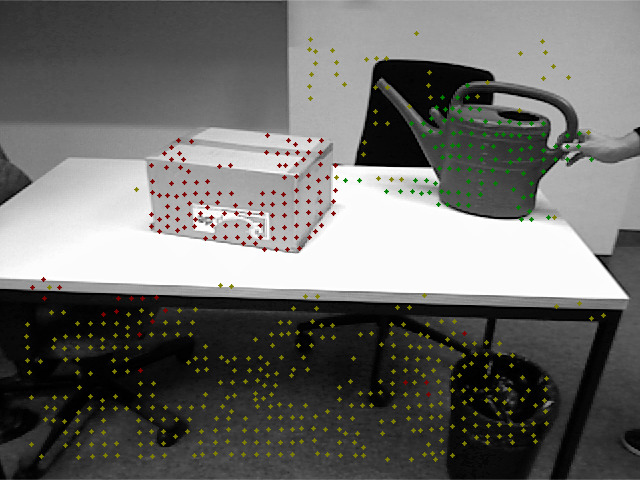
\includegraphics[width=0.48\linewidth] {evaluation/meth_cmp_bonn_wc/srsf_ped_sc}
   \label{fig:bonn_wc_c}
}
\subfigure[SRSF PED MC]{
   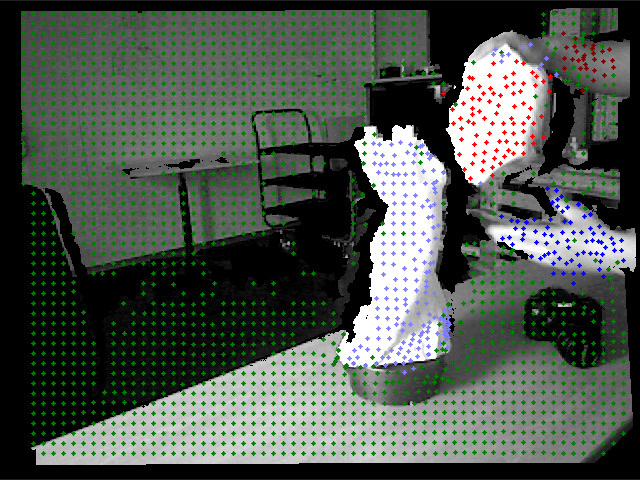
\includegraphics[width=0.48\linewidth] {evaluation/meth_cmp_bonn_wc/srsf_ped_mc}
   \label{fig:bonn_wc_d}   
}
\end{center}
\caption[Method Comparison]{Visualization of merged segmentations when comparing various methods}
\label{fig:bonn_watercan_method_cmp}
\end{figure}

\begin{figure}[H]
\begin{center}
\subfigure[LDOF PD SC]{
   \includegraphics[width=0.48\linewidth] {evaluation/meth_cmp_bonn_wc/ldof_pd_sc}
   \label{fig:bonn_wc_ed}
}
\subfigure[LDOF PD MC]{
   \includegraphics[width=0.48\linewidth] {evaluation/meth_cmp_bonn_wc/ldof_pd_mc}
   \label{fig:bonn_wc_f}   
}
\end{center}
\caption[Method Comparison 2]{Visualization of merged segmentations when comparing various methods}
\label{fig:bonn_watercan_method_cmp_2}
\end{figure}


\begin{table}[]
\centering
\begin{tabular}{|l|l|r|l|l|}
\hline
\multicolumn{5}{|c|}{Method Comparison, 12 fixed Clusters, Bonn Watercan}                        \\ \hline
              & \textbf{Density} & \textbf{Precission} & \textbf{Recall} & \textbf{F1 Score} \\ \hline
LDOF PD SC * & 0.44434 & 72.783 \%   & 66.1853 \%     & 69.3275 \%  \\ \hline
LDOF PD MC * & 0.44434 & 34.1727 \%   & 45.6731 \%     & 39.0947 \%  \\ \hline              
LDOF PED SC * & 0.43522 & 94.2955 \%   & 58.2015 \%     & 71.9770 \%  \\ \hline
LDOF PED MC * & 0.43522 & 64.4977 \%   & 81.0601 \%     & 71.8366 \%  \\ \hline
LDOF SD KL & 0.21094 & 84.4582 \%   & 70 \%     & 75.8336 \%  \\ \hline
LDOF SED KL & 0.21094 & 84.4582 \%   & 70 \%     & 75.8336 \%  \\ \hline
SRSF PD SC & 0.21094 & 84.4582 \%   & 70 \%     & 75.8336 \%  \\ \hline
SRSF PD MC & 0.21094 & 84.4582 \%   & 70 \%     & 75.8336 \%  \\ \hline
SRSF PED SC * & 0.20085 & 83.5144 \%   & 95.7385 \%     & 89.2096 \%  \\ \hline
SRSF PED MC * & 0.19889 & 92.9871 \%   & 70 \%     & 79.8725 \%  \\ \hline
SRSF SD KL & 0.21094 & 84.4582 \%   & 70 \%     & 75.8336 \%  \\ \hline
SRSF SED KL & 0.21094 & 84.4582 \%   & 70 \%     & 75.8336 \%  \\ \hline
\end{tabular}
\caption[Method Comparision Bonn Watercan]{My caption}
\label{tab:bonn_wc_methods}
\end{table}


explain the assumption of the datasets
explain what kind of segmentations have been generated and evaluated.







parameterspace exploration
running different similarity tasks




